% !TEX root = index.tex

\section{Gluing it Back Together}
\epigraph{The only way to learn math is to do math.}{Paul Halmos}
\begin{align*}
	\xymatrix@R-2pc{
	\U \ar@{~>}[r]          & \L^\bullet \ar@{~>}[r]     & \check H^*(X)                \\
	\mbox{Good cover of } X & \mbox{Cech Complex of } \U & \mbox{Cech Cohomology of } X
	}
\end{align*}
We now know enough theory to define the {Cech Cohomology} of a space. We'll start by defining it in an ad hoc manner and later try and understand it better.

Let $\U$ be a good cover of $X$ consisting of $n$ sets. In order to define the Cech Complex $\L^\bullet$ we need two things:
\begin{alignat*}{4}
	 & \mbox{vector spaces } &  & \qquad \L^k                          \\
	 & \mbox{linear maps }   &  & \qquad d^k: \L^k\rightarrow \L^{k+1}
\end{alignat*}

\begin{definition}
	The vector space $\L^k$ has dimension
	\begin{align*}
		\dim \L^k = \sum \limits_{|I| = k+1} \mbox{ number of connected components of } U_I
	\end{align*}
	where $I$ varies over the non-empty subsets of $[n]$.\footnote{Recall that to every subset $ I \subseteq [n]$ we can associate a set $U_I $ defined as $U_I := \bigcap_{i \in I} U_i$}
\end{definition}
\begin{definition}
	The linear map $d^k$ is a matrix whose \\
  \begin{tabular}{l l}
  rows & correspond to the connected components of all the $U_I$ with $|I|=k+2$ \\
  columns & correspond to the connected components of all the $U_J$ with $|J|=k+1$ \\
  $(i,j)^{th}$ entry & equals 1 if and only if the $i^{th}$ connected component in $U_I$ is a subset of \\
  & the $j^{th}$ connected component in $U_J$ (see examples).
  \end{tabular}
\end{definition}
\begin{definition}
	Define the \textbf{Cech Cohomology} $\check H^k(X)$ of $X$ to be the cohomology of the above cochain complex $\check H^k(\L)$.
\end{definition}

\begin{example}
	\label{ex:triangle_2}
	For the triangle with cover being the three sides $ \: \U = \{U_1, U_2, U_3\}$
	\begin{figure}[H]
		\centering
		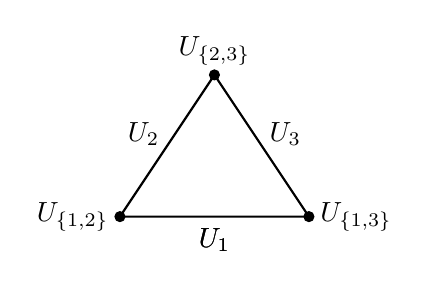
\begin{tikzpicture}[scale=0.6]
			%% vertices
			\draw[fill=black] (0,0) circle (3pt);
			\draw[fill=black] (4,0) circle (3pt);
			\draw[fill=black] (2,3) circle (3pt);
			%% vertex labels
			\node at (2,-0.5) {$U_1$};
			\node at (0.5,1.75) {$U_2$};
			\node at (3.5,1.75) {$U_3$};
			\node at (2,-0.5) {$U_1$};
			\node at (-1,0) {$U_{\{1,2\}}$};
			\node at (5,0) {$U_{\{1,3\}}$};
			\node at (2,3.5) {$U_{\{2,3\}}$};
			%%% edges
			\draw[thick] (0,0) -- (4,0) -- (2,3) -- (0,0);
		\end{tikzpicture}
		\caption{$\U = \{U_1, U_2, U_3\}$ is a good cover of the triangle, $U_{\{1,2\}}, U_{\{2,3\}}, U_{\{1,3\}}$ are the vertices, and $U_{\{1,2,3\}}$ is empty.}
		\label{fig:triangle_cech}
	\end{figure}
	\begin{align*}
		 & |I| = 0 &  & U_1, U_2, U_3                         &  & \L^0 = \F^3 \\
		 & |I| = 1 &  & U_{\{1,2\}}, U_{\{2,3\}}, U_{\{1,3\}} &  & \L^1 = \F^3
	\end{align*}
	We have inclusions $U_{\{1,2\}} \subseteq U_1$, $U_{\{1,2\}} \subseteq U_2$ etc. Hence the differential $d^0$ looks like
	\begin{center}
		\begin{tabular}{ l | c c c  }
			              & $U_1$ & $U_2$ & $U_3$ \\\hline
			$U_{\{1,2\}}$ & 1     & 1     & 0     \\
			$U_{\{2,3\}}$ & 0     & 1     & 1     \\
			$U_{\{1,3\}}$ & 1     & 0     & 1
		\end{tabular} $ = d^0$
	\end{center}
	So that
	\begin{align*}
		\L^\bullet
		 & =
		0 \rightarrow \F^3 \xrightarrow{\begin{bmatrix}1 & 1 & 0 \\0 & 1 & 1 \\ 1 & 0 & 1 \end{bmatrix}} \F^3 \rightarrow 0 \\
	\end{align*}
\end{example}

\begin{example}
	For the circle $S^1$ we can find a good cover consisting of semicircles $\: \U = \{U_1, U_2 \}$.
	\label{ex:circle_cech}
	\begin{figure}[H]
		\centering
		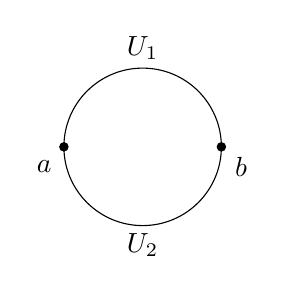
\begin{tikzpicture}[scale=0.5]
			%% vertices
			\draw (2,2) circle (2cm);
			\draw[fill=black] (0,2) circle (3pt);
			\draw[fill=black] (4,2) circle (3pt);
			\node at (2,4.5) {$U_1$};
			\node at (2,-0.5) {$U_2$};
			\node at (-0.5,1.5) {$a$};
			\node at (4.5,1.5) {$b$};
		\end{tikzpicture}
		\caption{$\{U_1, U_2\}$ is a good cover of the circle with $U_{\{1,2\}} = \{ a, b \}$}
		\label{fig:triangle_cech}
	\end{figure}
	\begin{align*}
		 & |I| = 0 &  & U_1, U_2               &  & \L^0 = \F^2 \\
		 & |I| = 1 &  & U_{\{1,2\}} = \{a, b\} &  & \L^1 = \F^2
	\end{align*}
	We have inclusions $\{ a \} \subseteq U_1$, $\{ a \} \subseteq U_2$ etc. Hence the differential $d^0$ looks like
	\begin{center}
		\begin{tabular}{ l | c c  }
			    & $U_1$ & $U_2$ \\\hline
			$a$ & 1     & 1     \\
			$b$ & 1     & 1
		\end{tabular} $ = d^0$
	\end{center}
	So that
	\begin{align*}
		\L^\bullet
		 & =
		0 \rightarrow \F^2 \xrightarrow{\begin{bmatrix}1 & 1  \\1 & 1 \end{bmatrix}} \F^2 \rightarrow 0
	\end{align*}
\end{example}
\newpage

\begin{ques}
	Compute the dimensions of the cohomologies in the above examples.
\end{ques}
Compute the dimensions of the cohomologies for the following spaces. Interpret your results topologically.

\begin{ques} $ $
	\begin{multicols}{2}
		\begin{enumerate}
			\item $ \R^n$
			\item A tree
			\item $d$ points in $\R^2$
			\item The bipartite graph $ K_{2,3}$
			\item $ \R^2 \setminus \{(0,0) \}$
			\item $ \R^2 \setminus \{(0,0), (1,0), \dots, (d,0) \}$ for some positive integer $ d$
			\item $ S^2 $ minus a point
			\item $ S^2 $ minus 2 points
		\end{enumerate}
	\end{multicols}
\end{ques}

\begin{ques} $ $
	\begin{enumerate}
		\item $S^1 \vee S^1$
		\item* Bouquet of $n$-circles\\
		      \begin{tikzpicture}[scale=0.6]
			      \begin{polaraxis}[grid=none, axis lines=none]
				      \addplot[mark=none,domain=0:360,samples=300] { abs(cos(8*x/2))};
			      \end{polaraxis}
		      \end{tikzpicture}
	\end{enumerate}
\end{ques}

\begin{ques} $ $
	\begin{enumerate}
		\item* $S^2$
		\item* $S^1 \vee S^2$
		\item** $S^1 \times S^1$ = torus (try to find a cover with 3 sets)
		\item*** $g$-holed torus
		\item Solid torus
	\end{enumerate}
\end{ques}

\newpage
The \emph{basis independent} way of defining the Cech Cohomology is as follows. Let $(U_{I_1}, U_{I_2}, \dots, U_{I_m})$ denote the non-empty sets $U_I$ with $|I| = k+1$. Then $L^k$ is the direct sum
\begin{align*}
	\L^k = \L(U_{I_1}) \oplus \L(U_{I_2}) \oplus \dots \oplus \L(U_{I_m})
\end{align*}
The differential maps $d^k$ are direct sums of the restriction maps $\res_{U_I \rightarrow U_J}$ for $|I|=k+1 , |J| = k+2$.
\begin{ques}*
	Prove this.
\end{ques}

\begin{ques}***
	Following is the proof of the fact that the Cech complex is indeed a cochain complex i.e. it satisfies $d^{k+1} \circ d^{k} = 0$:\\

  $\quad$ Consider subsets $J \subset I \subseteq [n]$ such that $k+1 = |J| = |I| - 2$ and $I = J \cup \{\alpha, \beta \}$. Let $J_{\alpha} := J \cup \{ \alpha \}$ and $J_{\beta} := J \cup \{ \beta \}$. Show that we have the following induced maps:
		\begin{align*}
	    J \subset J_\alpha \subset I \\
	      J \subset J_\beta \subset I
	  \end{align*}
		\begin{align*}
	    U_{I} \subset U_{J_\alpha} \subset U_{J} \\
	    U_{I} \subset U_{J_\beta} \subset U_{J}
	  \end{align*}
		\begin{align*}
			\phi_\alpha: \L(U_J) \xrightarrow{\res_{U_J \rightarrow U_{J_\alpha}}} \L(U_{J_\alpha}) \xrightarrow{\res_{U_{J_\alpha} \rightarrow U_{I}}} \L(U_I) \\
			\phi_\beta: 	\L(U_J) \xrightarrow{\res_{U_J \rightarrow U_{J_\beta}}} \L(U_{J_\beta}) \xrightarrow{\res_{U_{J_\beta} \rightarrow U_{I}}} \L(U_I)
		\end{align*}
		and $U_{I} = U_{J_\alpha} \cap U_{J_\beta}$, $U_{J} = U_{J_\alpha} \cup U_{J_\beta}$.
		Show that $d^{k+1} \circ d^{k}|_{\L(U_J)} = \phi_{\alpha} + \phi_{\beta}$. Argue that this implies $d^{k+1} \circ d^{k}|_{\L(U_J)} = 0$ and hence $d^{k+1} \circ d^{k} = 0$.
\end{ques}

Finally, notice that we're saying that for finding the Cech cohomology of $X$ we needed to choose a good open cover $\U$. It is a deep theorem that this choice does not matter. The only proof I know of this uses heavy homological algebra machinery.

\begin{thm}
	\label{thm:good_covers_theorem}
	If $ \U$, $\U'$ are \textbf{good covers} of $ X$ with associated Cech complexes $ \L^\bullet(\U)$ and $ \L^\bullet(\U')$ then
	\begin{align}
		H^i(\L(\U)) \cong  H^i(\L(\U'))
	\end{align}
	for all $ i \in \Z$ i.e. the cohomology of the Cech complex is independent of the good cover and hence is an invariant of the underlying space. Hence, we can define the Cech cohomology of $ X$ as
	\begin{align}
		\check H^i(X; \F) :=  H^i(\L(\U))
	\end{align}
	for any good cover $ \U$ of $ X$.
\end{thm}
